{\color{brown}\textbf{Ejemplo 3}}

En una tienda se venden rollos de papel higiénico. Cada rollo cuesta 2 dólares, pero hay la siguiente oferta:
Lleva 3 rollos de papel higiénico y paga solo 2.
Carlos compra 20 rollos del papel higiénico en oferta en esa tienda.\\
\textbf{¿Es correcto afirmar que pagó 40 dólares?}\\
Para resolver este problema utilizaremos una tabla de valores como la siguiente:

\begin{minipage}{.48\textwidth}
    \begin{figure}[H]
        \centering
        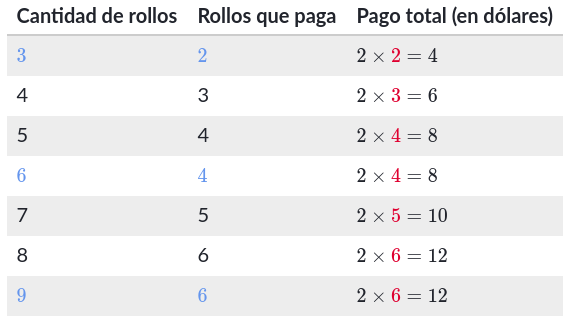
\includegraphics[width=\linewidth]{./Unidad 2/Images/tableS8L102.png}
    \end{figure}
\end{minipage}\hfill
\begin{minipage}{.48\textwidth}
    \begin{figure}[H]
        \centering
        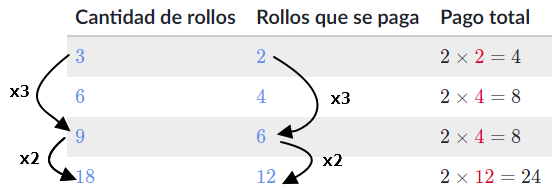
\includegraphics[width=\linewidth]{./Unidad 2/Images/tableS8L101.png}
    \end{figure}
\end{minipage}

Observamos que, si la cantidad de rollos es un múltiplo de 3, se cumple una relación proporcional
directa entre dicha cantidad y los rollos que deberá pagar. Como Carlos compra 20 rollos, podemos
observar que el múltiplo de 3 más cercano a 20 es 18. Así obtendremos la cantidad de rollos a pagar
luego de aplicar la oferta.\\

Gracias a la tabla, podemos observar que, llevando 18 rollos en oferta, solo pagará 12 rollos, es decir, 24 dólares.
Para comprar los 20 rollos, Carlos deberá pagar 2 rollos adicionales a un monto de 4 dólares.\\

Finalmente, por toda la compra pagará 24 dólares más 4 dólares adicionales, es decir, un total de 28 dólares.
Por tanto, la afirmación no es correcta. Carlos no pagó 40 dólares, sino 28.\\